% Relatório da Avaliação A2 — gerado por Modelagem_A2/gerar_relatorio_A2.py
% Compilar no Overleaf (pdfLaTeX) com o template oficial IEEEtran.
\documentclass[conference]{IEEEtran}
\IEEEoverridecommandlockouts
\usepackage[utf8]{inputenc}
\usepackage[T1]{fontenc}
\usepackage[brazil]{babel}
\usepackage{graphicx,amsmath,booktabs,url}
\graphicspath{{Modelagem_A2/figuras/}}
\begin{document}
\title{Vazamento de informação na triagem de laudos cardiológicos pediátricos: o que sobra quando o exame físico sai}
\author{\IEEEauthorblockN{Jamily Vieira, Júlia Souza, Yasmin Mageste}\IEEEauthorblockA{Instituto de Informática, Universidade Federal de Goiás\\Mineração de Dados --- Avaliação A2}\thanks{Código e dados para reprodução: \url{https://github.com/Julia-PS24/mineracao_de_dados} (random\_state = 42 em todas as etapas).}}
\maketitle
\begin{abstract}
Este trabalho avalia se o laudo de uma consulta de cardiologia pediátrica pode ser previsto a partir do que se conhece antes do exame especializado, usando 10.576 consultas de um ambulatório universitário. A análise exploratória identificou vazamento de informação: sopro, segunda bulha e pulsos são registrados no mesmo exame que produz o rótulo, e 96\% das consultas com sopro sistólico têm laudo anormal. Esses 10 atributos foram excluídos, restando 37. Quatro algoritmos foram comparados em validação cruzada dentro do treino, com o pré-processamento reajustado em cada dobra, e avaliados uma única vez num teste de 2.116 consultas. A área sob a curva ROC cai de 0,95 com o exame físico para 0,78 sem ele: a diferença mede o vazamento, não capacidade preditiva. O motivo do encaminhamento responde por quase toda a capacidade restante, e 73\% dos laudos anormais não detectados vêm de pedidos de rotina, sem suspeita prévia.
\end{abstract}
\begin{IEEEkeywords}
mineração de dados, classificação, vazamento de informação, triagem clínica, cardiologia pediátrica
\end{IEEEkeywords}
\section{Introdução}
Serviços públicos de cardiologia pediátrica recebem mais encaminhamentos do que conseguem atender com prontidão. Uma ferramenta capaz de ordenar a fila pela probabilidade de laudo alterado teria valor prático: adiantaria a avaliação das crianças com maior risco sem exigir recursos adicionais. A pergunta deste trabalho é se essa ordenação é possível com a informação que existe \textit{antes} da consulta especializada.

A base utilizada reúne 12.873 consultas de um ambulatório universitário, reduzidas a 10.576 após a limpeza realizada na etapa anterior do estudo, das quais 4.485 (42,4\%) têm laudo anormal. A tarefa de mineração é a classificação binária desse desfecho.

A principal dificuldade não é o algoritmo, e sim decidir quais atributos podem ser usados. Vários deles descrevem o próprio exame cujo resultado se quer prever, e um modelo que os utilize alcança desempenho elevado sem ter utilidade alguma: prevê o laudo com o laudo. O vazamento de informação é um erro de formulação que a validação cruzada não detecta, porque não decorre de sobreajuste [8]. Este relatório identifica os atributos nessa condição, exclui-os, mede quanto o desempenho cai com a exclusão e examina o que resta.

Todo o código, com semente aleatória fixa, está no repositório indicado na primeira página, implementado em Python com scikit-learn [1], pandas [2] e matplotlib [3]. Quatro algoritmos foram comparados: um piso trivial, um modelo linear interpretável e dois conjuntos de árvores de decisão.

\section{Dados e Análise Exploratória}
Cada linha da base corresponde a uma consulta e reúne dados demográficos (idade e sexo), medidas antropométricas (peso, altura e índice de massa corporal), sinais vitais (frequência cardíaca e pressão arterial), sintomas relatados, o motivo do encaminhamento e os achados do exame físico realizado pelo cardiologista. O alvo é o laudo final, normal ou anormal. O desbalanceamento é leve --- 42,4\% de laudos anormais contra 57,6\% de normais --- e não justifica reamostragem; justifica, porém, não interpretar a acurácia isoladamente, já que prever sempre ``normal'' alcança 0,576.

\subsection{O atributo com vazamento de informação}
O rótulo é a conclusão do cardiologista após o exame. Sopro, segunda bulha e pulsos são exatamente o que ele ausculta e palpa nesse mesmo exame, e por isso não estão disponíveis no momento em que uma triagem precisaria da previsão. A Fig. 1 mostra a dimensão do problema: entre as 4.144 consultas com algum achado alterado, a proporção de laudos anormais chega a 96\% no sopro sistólico, enquanto as 6.432 consultas sem nenhuma alteração ficam em 8,6\%. A etapa anterior do estudo havia medido para o sopro um V de Cramér de 0,84, valor que nenhum atributo anterior à consulta alcança.

Os 10 atributos codificados a partir desses três achados foram excluídos da análise. O critério é a origem da informação, não a força da associação: pulsos e segunda bulha alteram-se em poucas consultas, mas são anotados no mesmo ato clínico e sairiam pelo mesmo motivo. Restam 37 atributos de entrada.

O motivo do encaminhamento foi mantido, e essa decisão merece justificativa, já que o encaminhamento por sopro é o atributo mais importante dos modelos. Ele é escrito pelo médico que encaminha, antes da consulta, e portanto está disponível na triagem. Além disso, não reproduz o achado do exame: das 2.122 crianças encaminhadas por sopro, o cardiologista o confirmou em 1.653 (78\%), e as 469 em que não confirmou têm apenas 11,7\% de laudos anormais; na direção oposta, das 3.994 consultas com sopro no exame, somente 41\% vinham encaminhadas por sopro. A suspeita prévia é informativa e imperfeita --- o que se espera de um atributo legítimo.

\begin{figure}[!t]
\centering
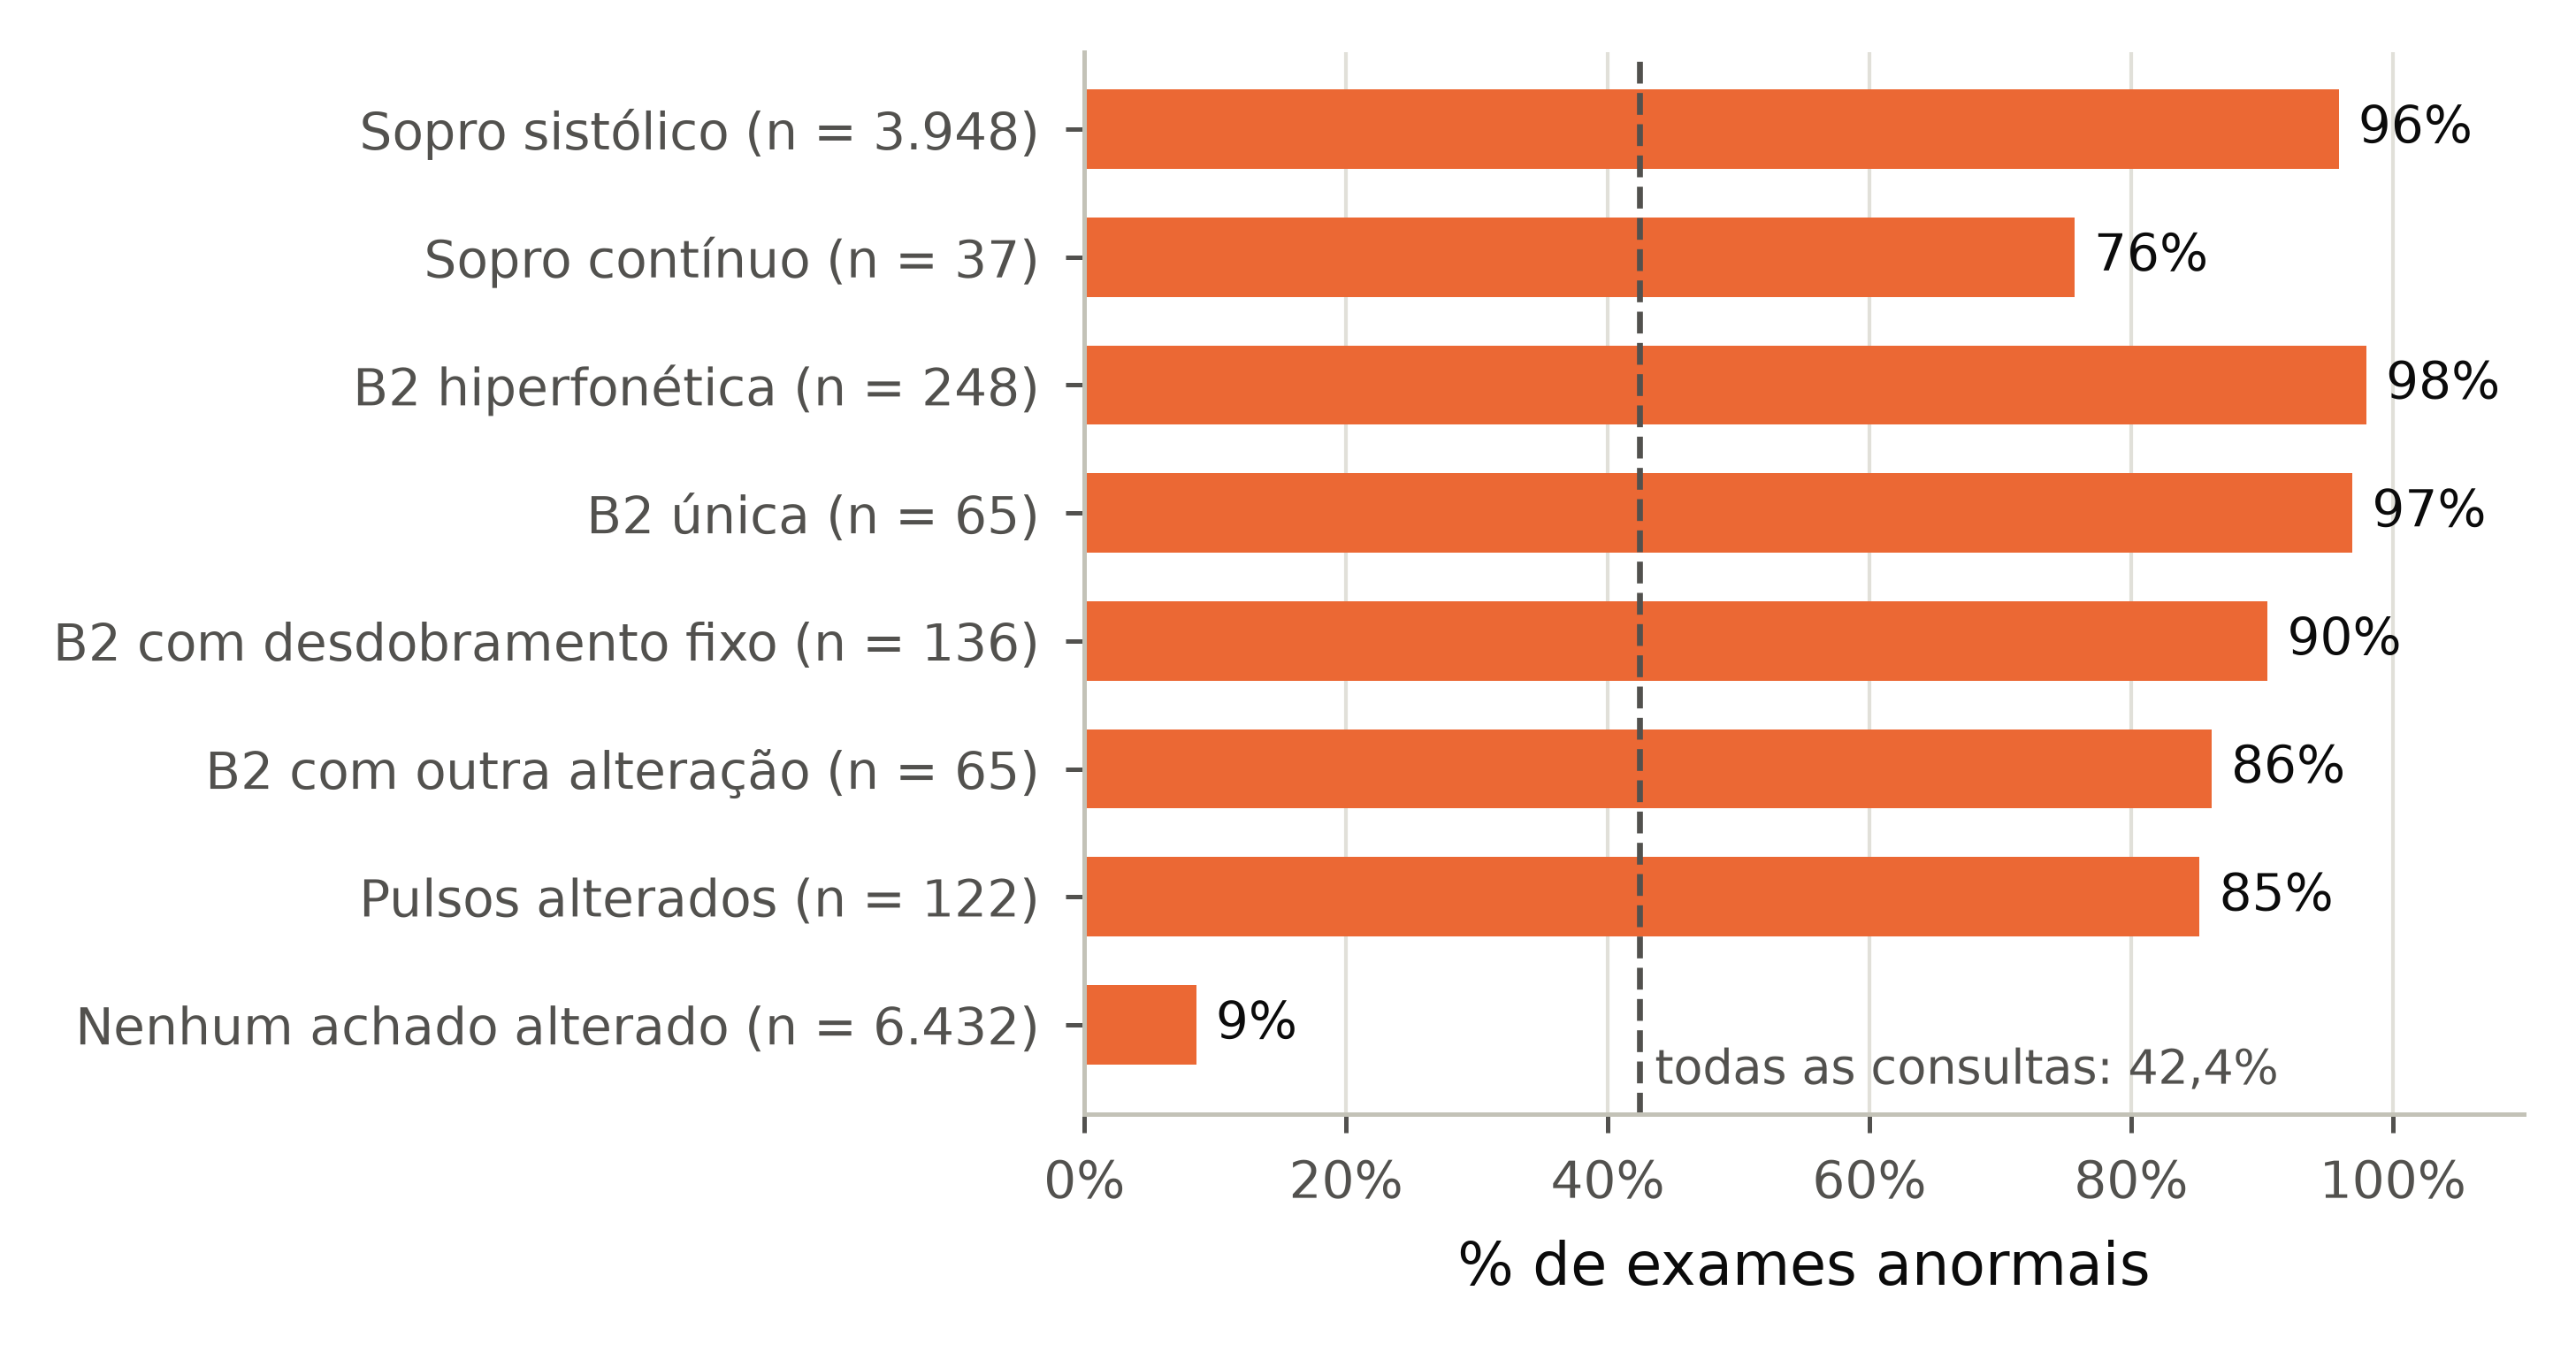
\includegraphics[width=\columnwidth]{fig1_vazamento_exame_fisico}
\caption{Proporção de laudos anormais em cada achado do exame físico, na base limpa. A linha tracejada marca a proporção do conjunto completo. Achados registrados no mesmo exame que produz o rótulo separam as classes quase perfeitamente, sinal de vazamento de informação.}
\label{fig:fig1_vazamento_exame_fisico}
\end{figure}
Entre os atributos efetivamente utilizáveis, dois se destacam (Fig. 2). A idade concentra o risco: a proporção de laudos anormais cai de 61,2\% no primeiro ano de vida para 27,9\% entre 15 e 19 anos. O motivo do encaminhamento separa ainda mais: as consultas por cardiopatia já estabelecida chegam a 71,2\% de laudos anormais, contra 25,2\% nos pedidos de parecer cardiológico, que são o motivo mais frequente da base (4.795 consultas).

\begin{figure}[!t]
\centering
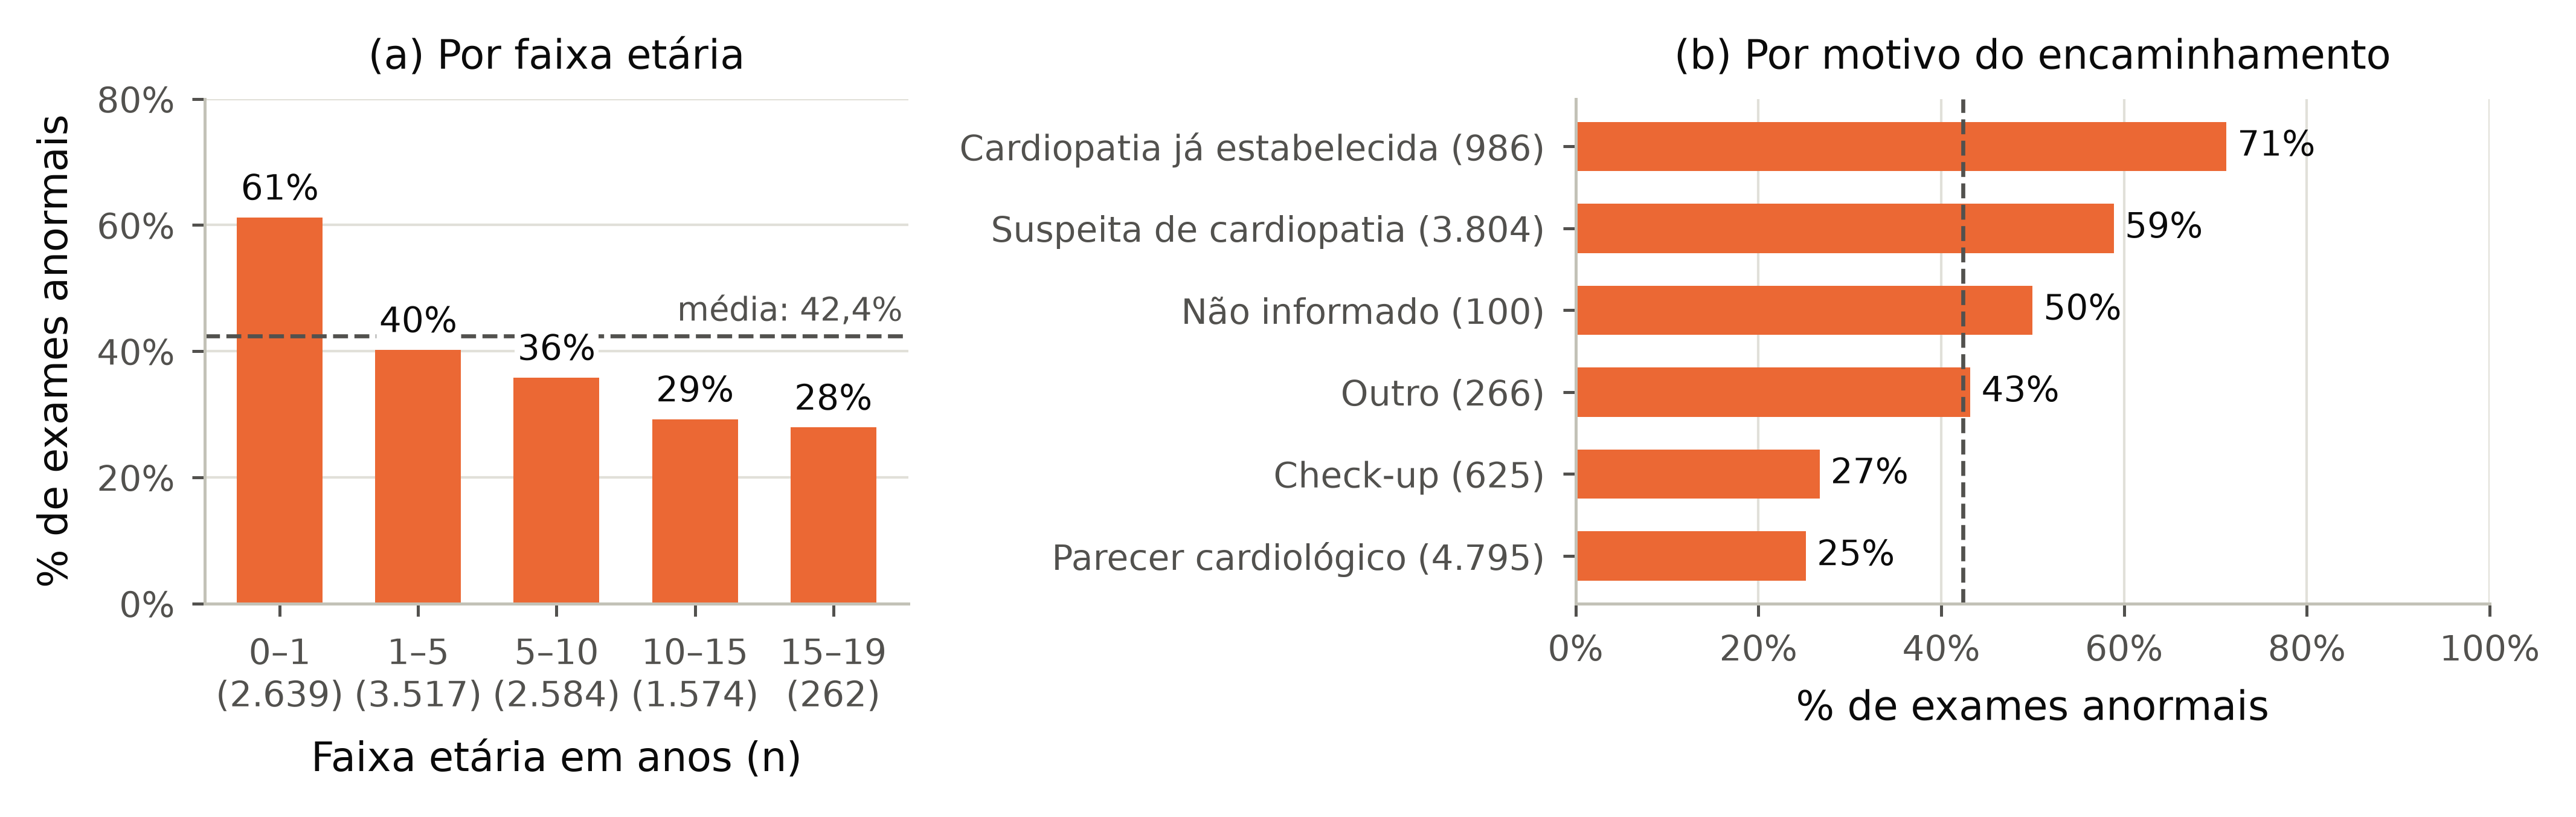
\includegraphics[width=\columnwidth]{fig2_alvo_idade_motivo}
\caption{Proporção de laudos anormais por faixa etária (a) e por motivo principal do encaminhamento (b), na base limpa, com o número de consultas entre parênteses. São as duas informações anteriores à consulta que mais pesam nos modelos.}
\label{fig:fig2_alvo_idade_motivo}
\end{figure}
\section{Metodologia}
\subsection{Pré-processamento}
O pré-processamento herdado da etapa anterior compreende: imputação de frequência cardíaca, pressão arterial e índice de massa corporal pela mediana da faixa etária; padronização desses sinais vitais dentro da faixa etária, para separar o efeito da variável do efeito da idade; transformação logarítmica da idade antes da padronização, o que reduz a assimetria de 0,76 para $-$0,25; exclusão de peso e altura, redundantes com a idade (correlação de Spearman de 0,97 e 0,99); codificação da pressão arterial percentilar, classificada segundo o Fourth Report [5], como variável ordinal acompanhada de dois indicadores de ausência; e agrupamento de categorias com menos de 30 casos. O índice de massa corporal segue as curvas de crescimento do CDC [4], e a faixa etária considerada vai de 0 a 19 anos, limite usual da pediatria [6].

O ponto metodologicamente relevante é \textit{quando} esse ajuste acontece. Medianas, médias, desvios-padrão, modas e a lista de categorias frequentes são estatísticas aprendidas dos dados; calculá-las sobre a base inteira antes de separar treino e validação transfere informação de um conjunto para o outro. Para evitá-lo, o pré-processador foi implementado como transformador do scikit-learn [1] e colocado em um \textit{pipeline}, de modo que é reajustado dentro de cada dobra, usando somente as linhas de ajuste daquela dobra.

\subsection{Protocolo de validação}
A base foi dividida em 8.460 consultas de treino e 2.116 de teste (42,4\% de laudos anormais em ambos), tomando uma das cinco partições de uma divisão estratificada --- e não um corte aleatório isolado. Todas as decisões (hiperparâmetros, escolha do modelo e limiar de decisão) foram tomadas por validação cruzada de cinco dobras estratificadas \textit{dentro do treino}. O teste foi aberto uma única vez, após todas as decisões, e nenhum resultado dele realimentou escolha alguma.

A etapa anterior previa agrupar a divisão por uma chave construída a partir da data de atendimento e da data de nascimento, supondo identificar o mesmo paciente. A verificação realizada aqui não sustenta a suposição: dos 160 grupos com mais de uma consulta, 31 reúnem registros de sexos diferentes e 42 reúnem laudos diferentes --- são crianças distintas atendidas no mesmo dia. A base não possui identificador de paciente, de modo que cada consulta é tratada como observação independente, e a impossibilidade de descartar consultas repetidas consta entre as limitações do estudo.

Como uma estimativa obtida em um único conjunto de teste depende da partição sorteada, o resultado principal foi confirmado por validação cruzada aninhada, com cinco dobras externas de avaliação e três internas de escolha de hiperparâmetros, aplicada às 10.576 consultas [7]. Nesse protocolo nenhuma observação participa ao mesmo tempo da escolha e da avaliação, e a estimativa não depende de um corte específico.

\subsection{Algoritmos e métricas}
Quatro algoritmos foram comparados. A classe majoritária fixa o piso: prevê sempre ``normal'' e não aprende nada. A regressão logística é o modelo simples exigido --- linear, aditivo e auditável coeficiente a coeficiente. A floresta aleatória [9] e o \textit{gradient boosting} por histogramas [10] são os modelos complexos, capazes de representar efeitos não lineares e interações: a primeira combina centenas de árvores ajustadas a amostras distintas, reduzindo variância; o segundo ajusta árvores pequenas em sequência, cada uma corrigindo o erro acumulado das anteriores, reduzindo viés. Os hiperparâmetros foram escolhidos por busca em grade sobre a área sob a curva ROC média das dobras (57 combinações no total), sempre dentro do treino.

A área sob a curva ROC é a métrica de seleção, por não depender do limiar de decisão e medir diretamente a qualidade da ordenação, que é o uso pretendido. Entre as métricas que dependem de limiar, a sensibilidade na classe anormal recebe prioridade clínica: deixar de sinalizar uma criança com alteração cardíaca é mais grave do que um encaminhamento desnecessário. O limiar foi fixado, para cada modelo, no maior valor que alcança sensibilidade de 0,80 nas previsões \textit{out-of-fold} do treino, e só então aplicado ao teste. A importância dos atributos foi medida por permutação, e não pela redução de impureza das árvores, que favorece atributos com muitos valores distintos; a permutação foi feita também por grupo temático, porque atributos que descrevem a mesma informação se substituem mutuamente quando embaralhados um a um.

\section{Resultados e Discussão}
\begin{table}[!t]
\caption{Desempenho no cenário com 37 atributos. A coluna de validação cruzada traz a média e o desvio-padrão das cinco dobras do treino; as demais referem-se ao conjunto de teste (2.116 consultas), com intervalos de 95\% por reamostragem \textit{bootstrap}. Sensibilidade, especificidade e F1 usam o limiar fixado no treino.}
\label{tab:tabela_comparativa}
\centering
\small
\begin{tabular}{llccccc}
\toprule
modelo & AUC val. cruz. & AUC teste & IC 95\% & sens. & espec. & F1 \\
\midrule
Classe majoritária & 0,500 ± 0,000 & 0,500 & --- & --- & --- & --- \\
Logística & 0,764 ± 0,008 & 0,792 & 0,772 a 0,811 & 0,821 & 0,574 & 0,684 \\
Random forest & 0,775 ± 0,013 & 0,803 & 0,784 a 0,821 & 0,810 & 0,614 & 0,694 \\
Gradient boosting & 0,777 ± 0,015 & 0,802 & 0,784 a 0,821 & 0,810 & 0,624 & 0,698 \\
\bottomrule
\end{tabular}
\end{table}
Os três modelos superam com folga o piso da classe majoritária, e a diferença entre eles é pequena (Tabela I). Na validação cruzada, que é o critério de seleção, o gradient boosting alcança 0,777 contra 0,764 da regressão logística, uma vantagem de 0,012 com desvio entre dobras de 0,015. No teste, a reamostragem pareada \textit{bootstrap} [11] --- em que os dois modelos são avaliados nas mesmas consultas sorteadas --- confirma que a vantagem é consistente: a diferença é positiva em 98,0\% das reamostragens. Já a diferença entre os dois modelos complexos é indistinguível de zero, com intervalo de -0,007 a 0,005.

A estimativa do teste (0,802) é mais otimista que a da validação cruzada (0,777), o que indica uma partição favorável, não ganho real. A validação cruzada aninhada sobre as 10.576 consultas, que não depende de um corte único, devolve 0,786 ± 0,013 --- valor intermediário e o mais conservador dos três. É esse o número que o trabalho adota como desempenho esperado.

\begin{figure}[!t]
\centering
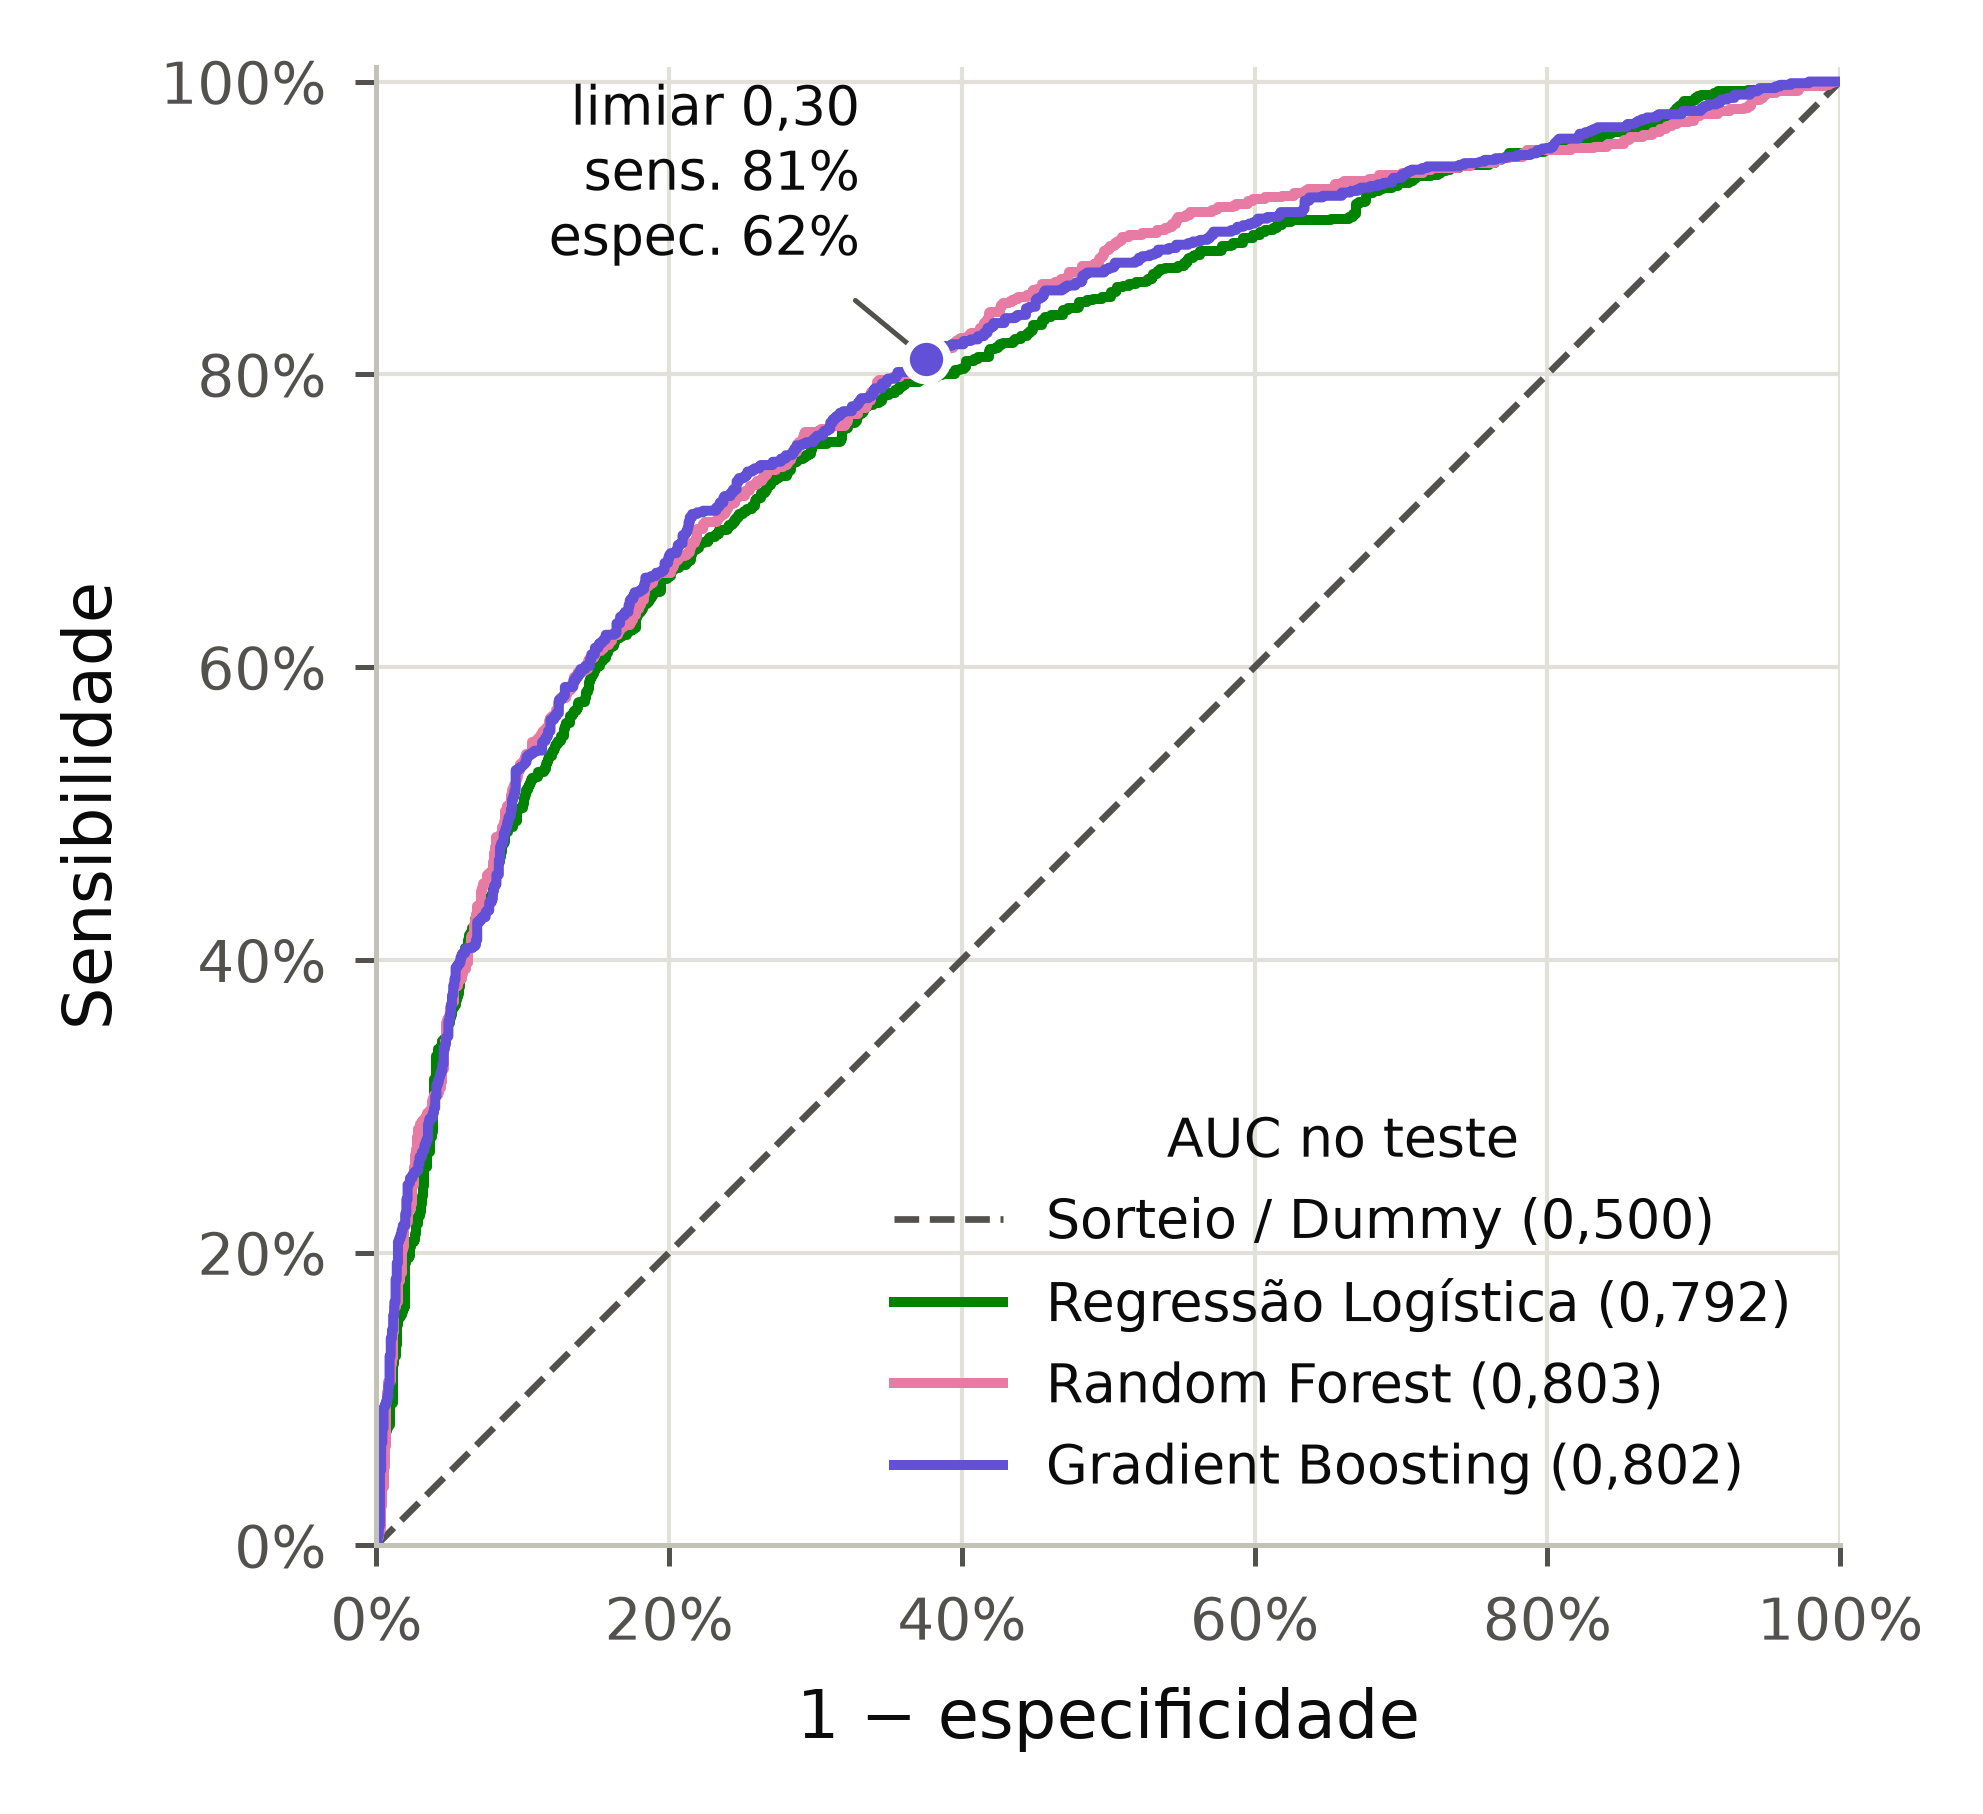
\includegraphics[width=\columnwidth]{fig4_roc_teste}
\caption{Curvas ROC no conjunto de teste. A diagonal corresponde ao desempenho de um sorteio. O ponto destacado marca o limiar fixado no treino para o modelo escolhido. As três curvas praticamente se sobrepõem: a vantagem dos modelos complexos não se concentra em nenhuma faixa de limiar.}
\label{fig:fig4_roc_teste}
\end{figure}
\subsection{O custo de excluir o exame físico}
A Fig. 4 responde à pergunta central. Com os achados do exame físico incluídos, a área sob a curva ROC do gradient boosting é 0,950; sem eles, 0,777. A queda de 0,174 não mede perda de capacidade preditiva: mede o quanto o laudo estava escrito dentro daqueles atributos. Um modelo com 0,95 de área sob a curva seria reportado como excelente e seria inútil, porque exige, para funcionar, justamente a informação que a triagem não tem. Retirar também o motivo do encaminhamento reduz o desempenho a 0,674, o que delimita o que se pode esperar usando apenas o que é medido na própria consulta.

\begin{figure}[!t]
\centering
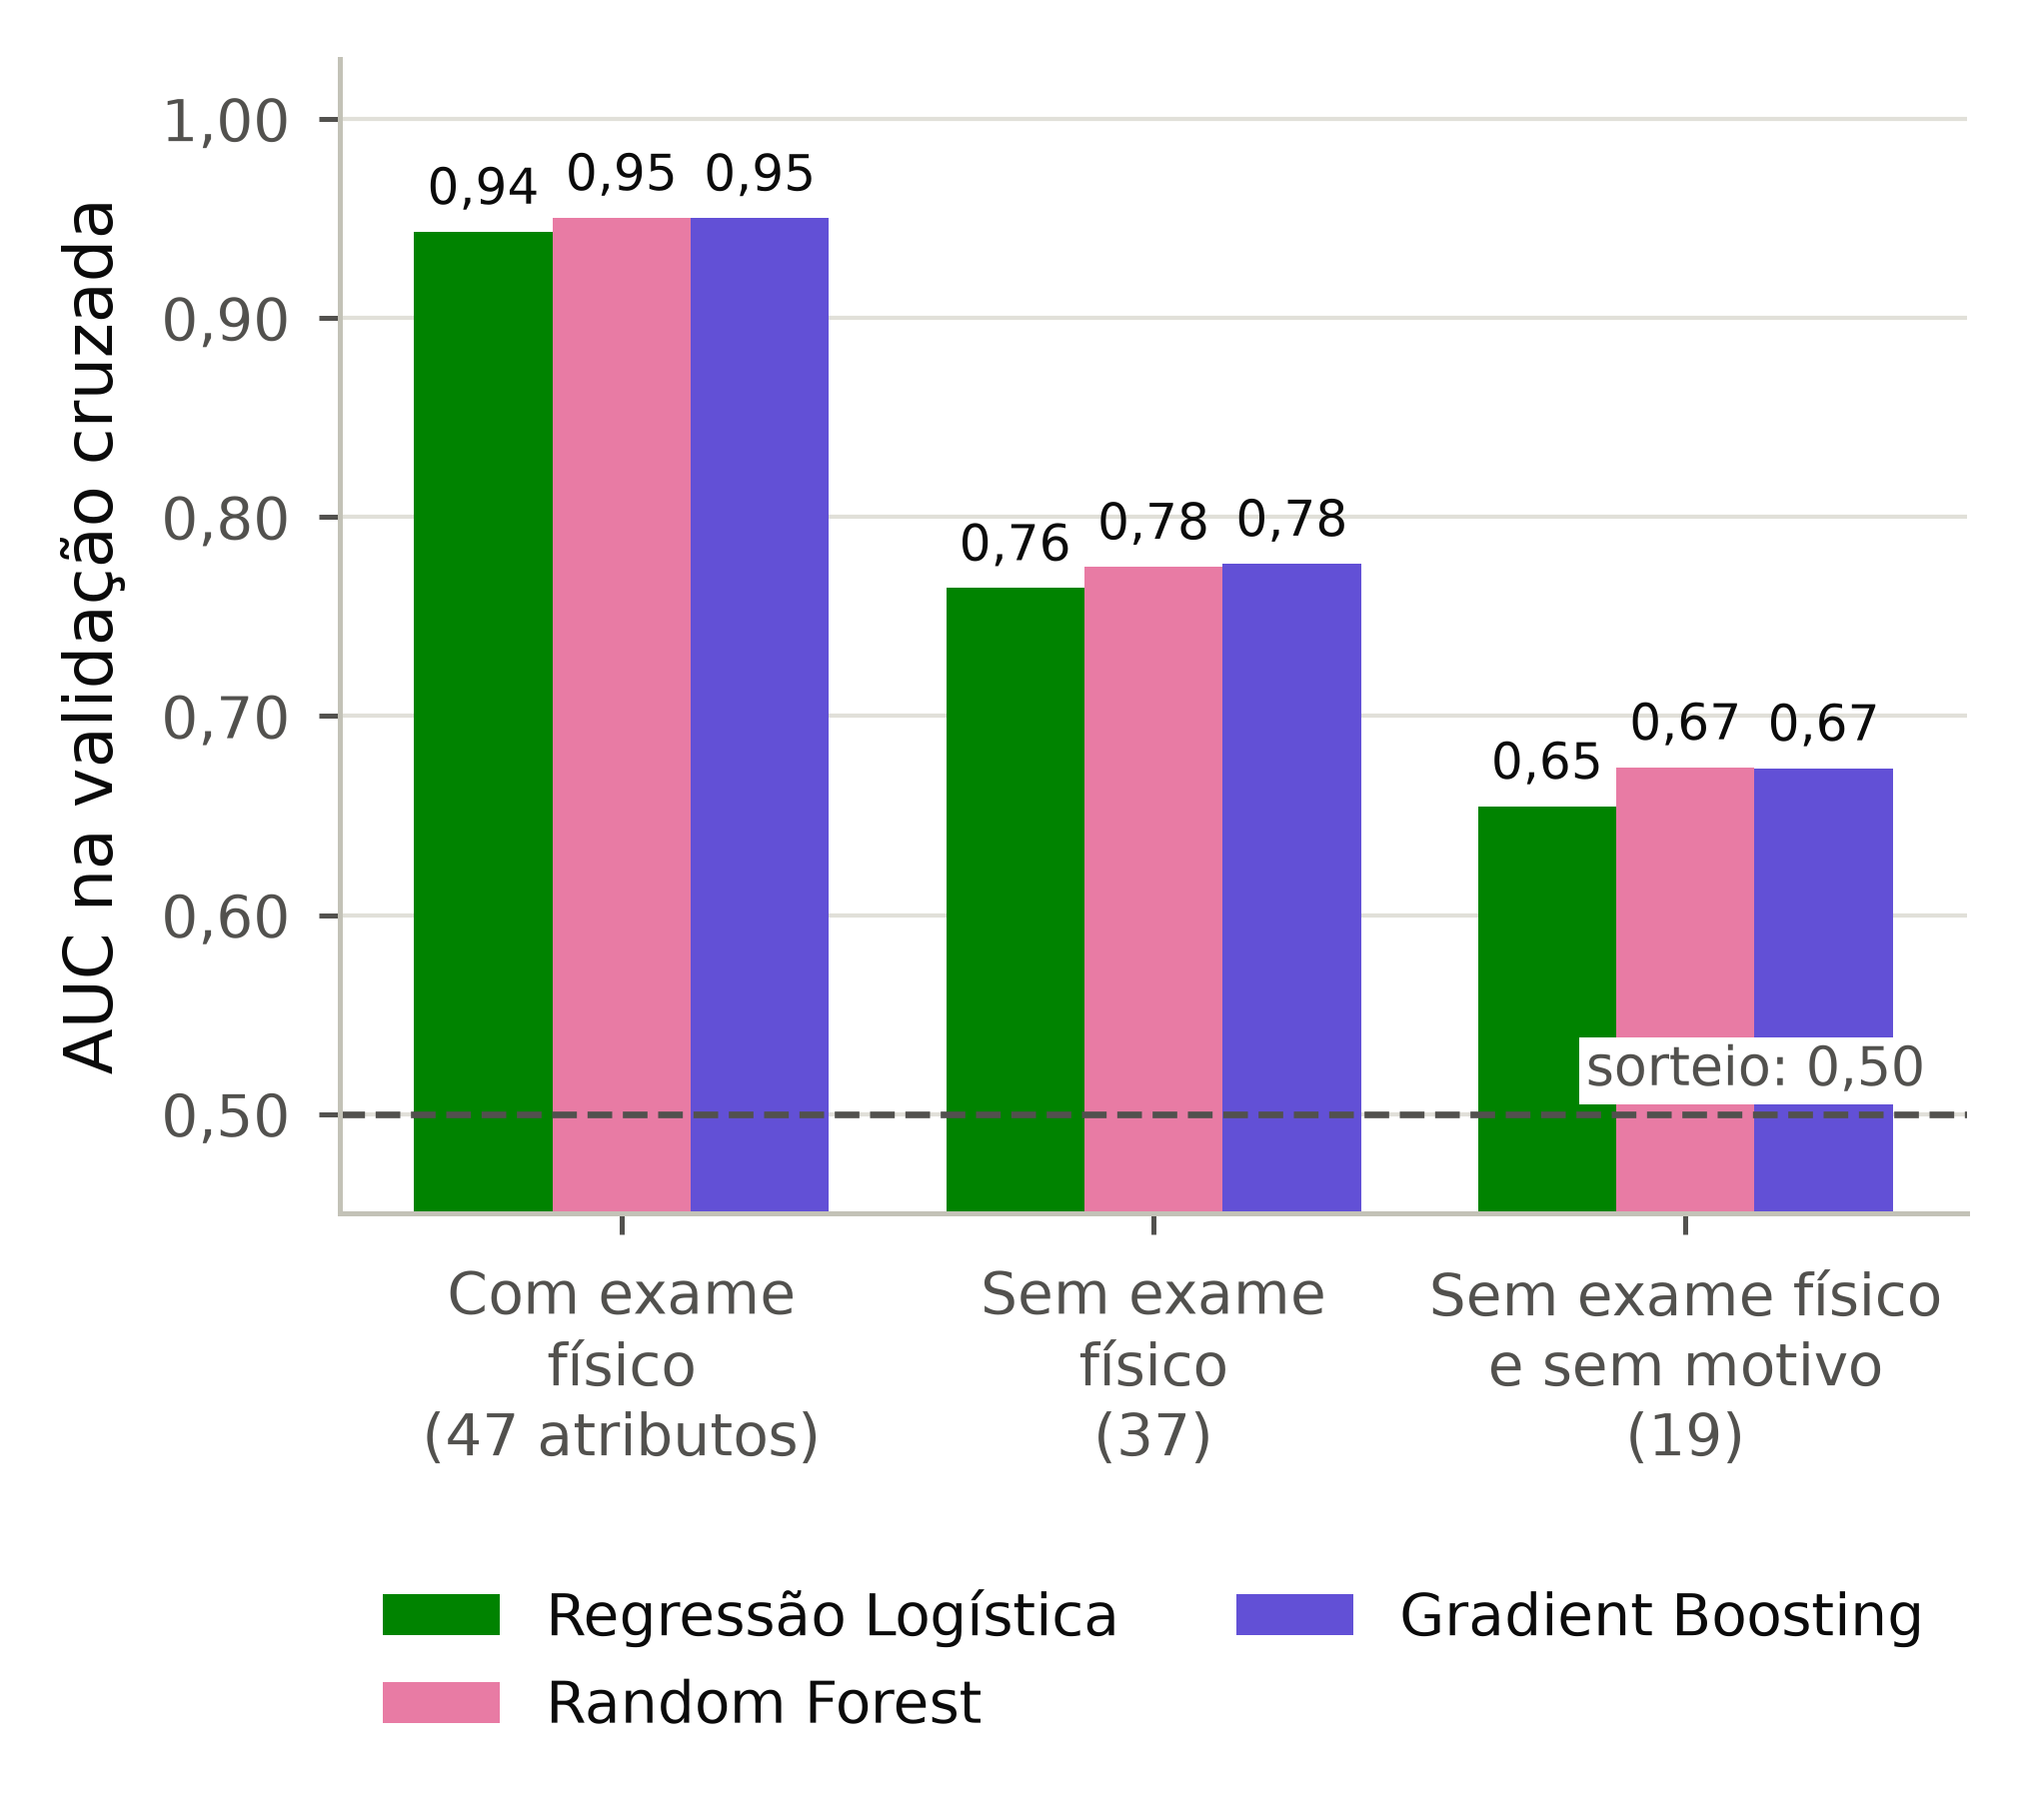
\includegraphics[width=\columnwidth]{fig3_regua_vazamento}
\caption{Área sob a curva ROC na validação cruzada do treino, por conjunto de atributos. O primeiro grupo de barras inclui os achados do exame físico e serve apenas de régua para medir o vazamento; o segundo é o cenário adotado; o terceiro remove também o motivo do encaminhamento.}
\label{fig:fig3_regua_vazamento}
\end{figure}
\subsection{Análise dos erros}
No limiar fixado no treino (0,30), o gradient boosting encontra 727 dos 897 laudos anormais do teste (81,0\%) e deixa passar 170; entre os 1.219 laudos normais, prioriza 458 (37,6\%) e libera 761. A assimetria é deliberada: há cerca de 2,7 falsos alarmes por laudo anormal perdido, consequência de exigir sensibilidade alta. A fila priorizada reúne 1.185 consultas, das quais 61,4\% são anormais; a fila liberada reúne 931, com 18,3\% de anormais --- menos da metade da proporção da base.

\begin{table}[!t]
\caption{Matriz de confusão do modelo escolhido no conjunto de teste, no limiar fixado no treino. Os percentuais são por linha, isto é, sobre o total de cada classe real.}
\label{tab:matriz_confusao}
\centering
\small
\begin{tabular}{llc}
\toprule
Gradient Boosting, limiar 0,30 & Liberado (previsto Normal) & Priorizado (previsto Anormal) \\
\midrule
Real: Normal & 761 (62,4\%) & 458 (37,6\%) \\
Real: Anormal & 170 (19,0\%) & 727 (81,0\%) \\
\bottomrule
\end{tabular}
\end{table}
Exigir mais sensibilidade custa caro, e de forma não linear. Nas previsões \textit{out-of-fold} do treino, passar de sensibilidade 0,75 para 0,80 eleva a fração de crianças priorizadas de 52,8\% para 59,7\%; alcançar 0,90 exigiria priorizar 76,9\% --- a triagem quase deixaria de triar. O ponto de operação é, portanto, uma decisão clínica e não estatística; o modelo entrega a curva inteira, e o valor adotado aqui é uma convenção de trabalho.

Os erros não se distribuem por igual, e é aí que está a parte interessante. Por faixa etária (Tabela III), a sensibilidade cai de 0,96 no primeiro ano de vida para 0,46 entre 15 e 19 anos, enquanto a especificidade faz o caminho inverso, de 0,31 para 0,95. O modelo acompanha a prevalência de cada faixa: prioriza quase todos os bebês, entre os quais 60,0\% têm laudo anormal, e quase ninguém entre os adolescentes.

\begin{table}[!t]
\caption{Desempenho do modelo escolhido por faixa etária, no conjunto de teste e no limiar fixado no treino. A última coluna traz o número de laudos anormais não detectados em cada faixa.}
\label{tab:erros_por_faixa}
\centering
\small
\begin{tabular}{llcccc}
\toprule
faixa (anos) & n & \% An. & sens. & espec. & An. perdidos \\
\midrule
0--1 & 543 & 60,0 & 0,963 & 0,313 & 12 \\
1--5 & 696 & 41,8 & 0,804 & 0,635 & 57 \\
5--10 & 515 & 35,3 & 0,670 & 0,667 & 60 \\
10--15 & 310 & 27,4 & 0,600 & 0,787 & 34 \\
15--19 & 52 & 25,0 & 0,462 & 0,949 & 7 \\
\bottomrule
\end{tabular}
\end{table}
Mais revelador, porém, é o motivo do encaminhamento. O desempenho acompanha a suspeita que vem no encaminhamento (Fig. 5): nas 178 consultas por cardiopatia já estabelecida, a sensibilidade é de 0,98, enquanto nas 970 consultas de parecer cardiológico, que têm apenas 24,4\% de laudos anormais, ela cai para 0,48. Essas últimas concentram 124 dos 170 laudos anormais não detectados (73\%).

A leitura clínica é direta e constitui o principal achado do trabalho: o modelo funciona como um resumo quantitativo do encaminhamento e da idade. Ordena bem quem já chega com suspeita e falha justamente onde a suspeita não existe --- nos pedidos de rotina, em que a alteração só aparece no exame. Uma triagem automatizada desse tipo adiantaria crianças que já seriam priorizadas pela leitura do encaminhamento, e acrescentaria pouco onde mais se precisaria dela.

\begin{figure}[!t]
\centering
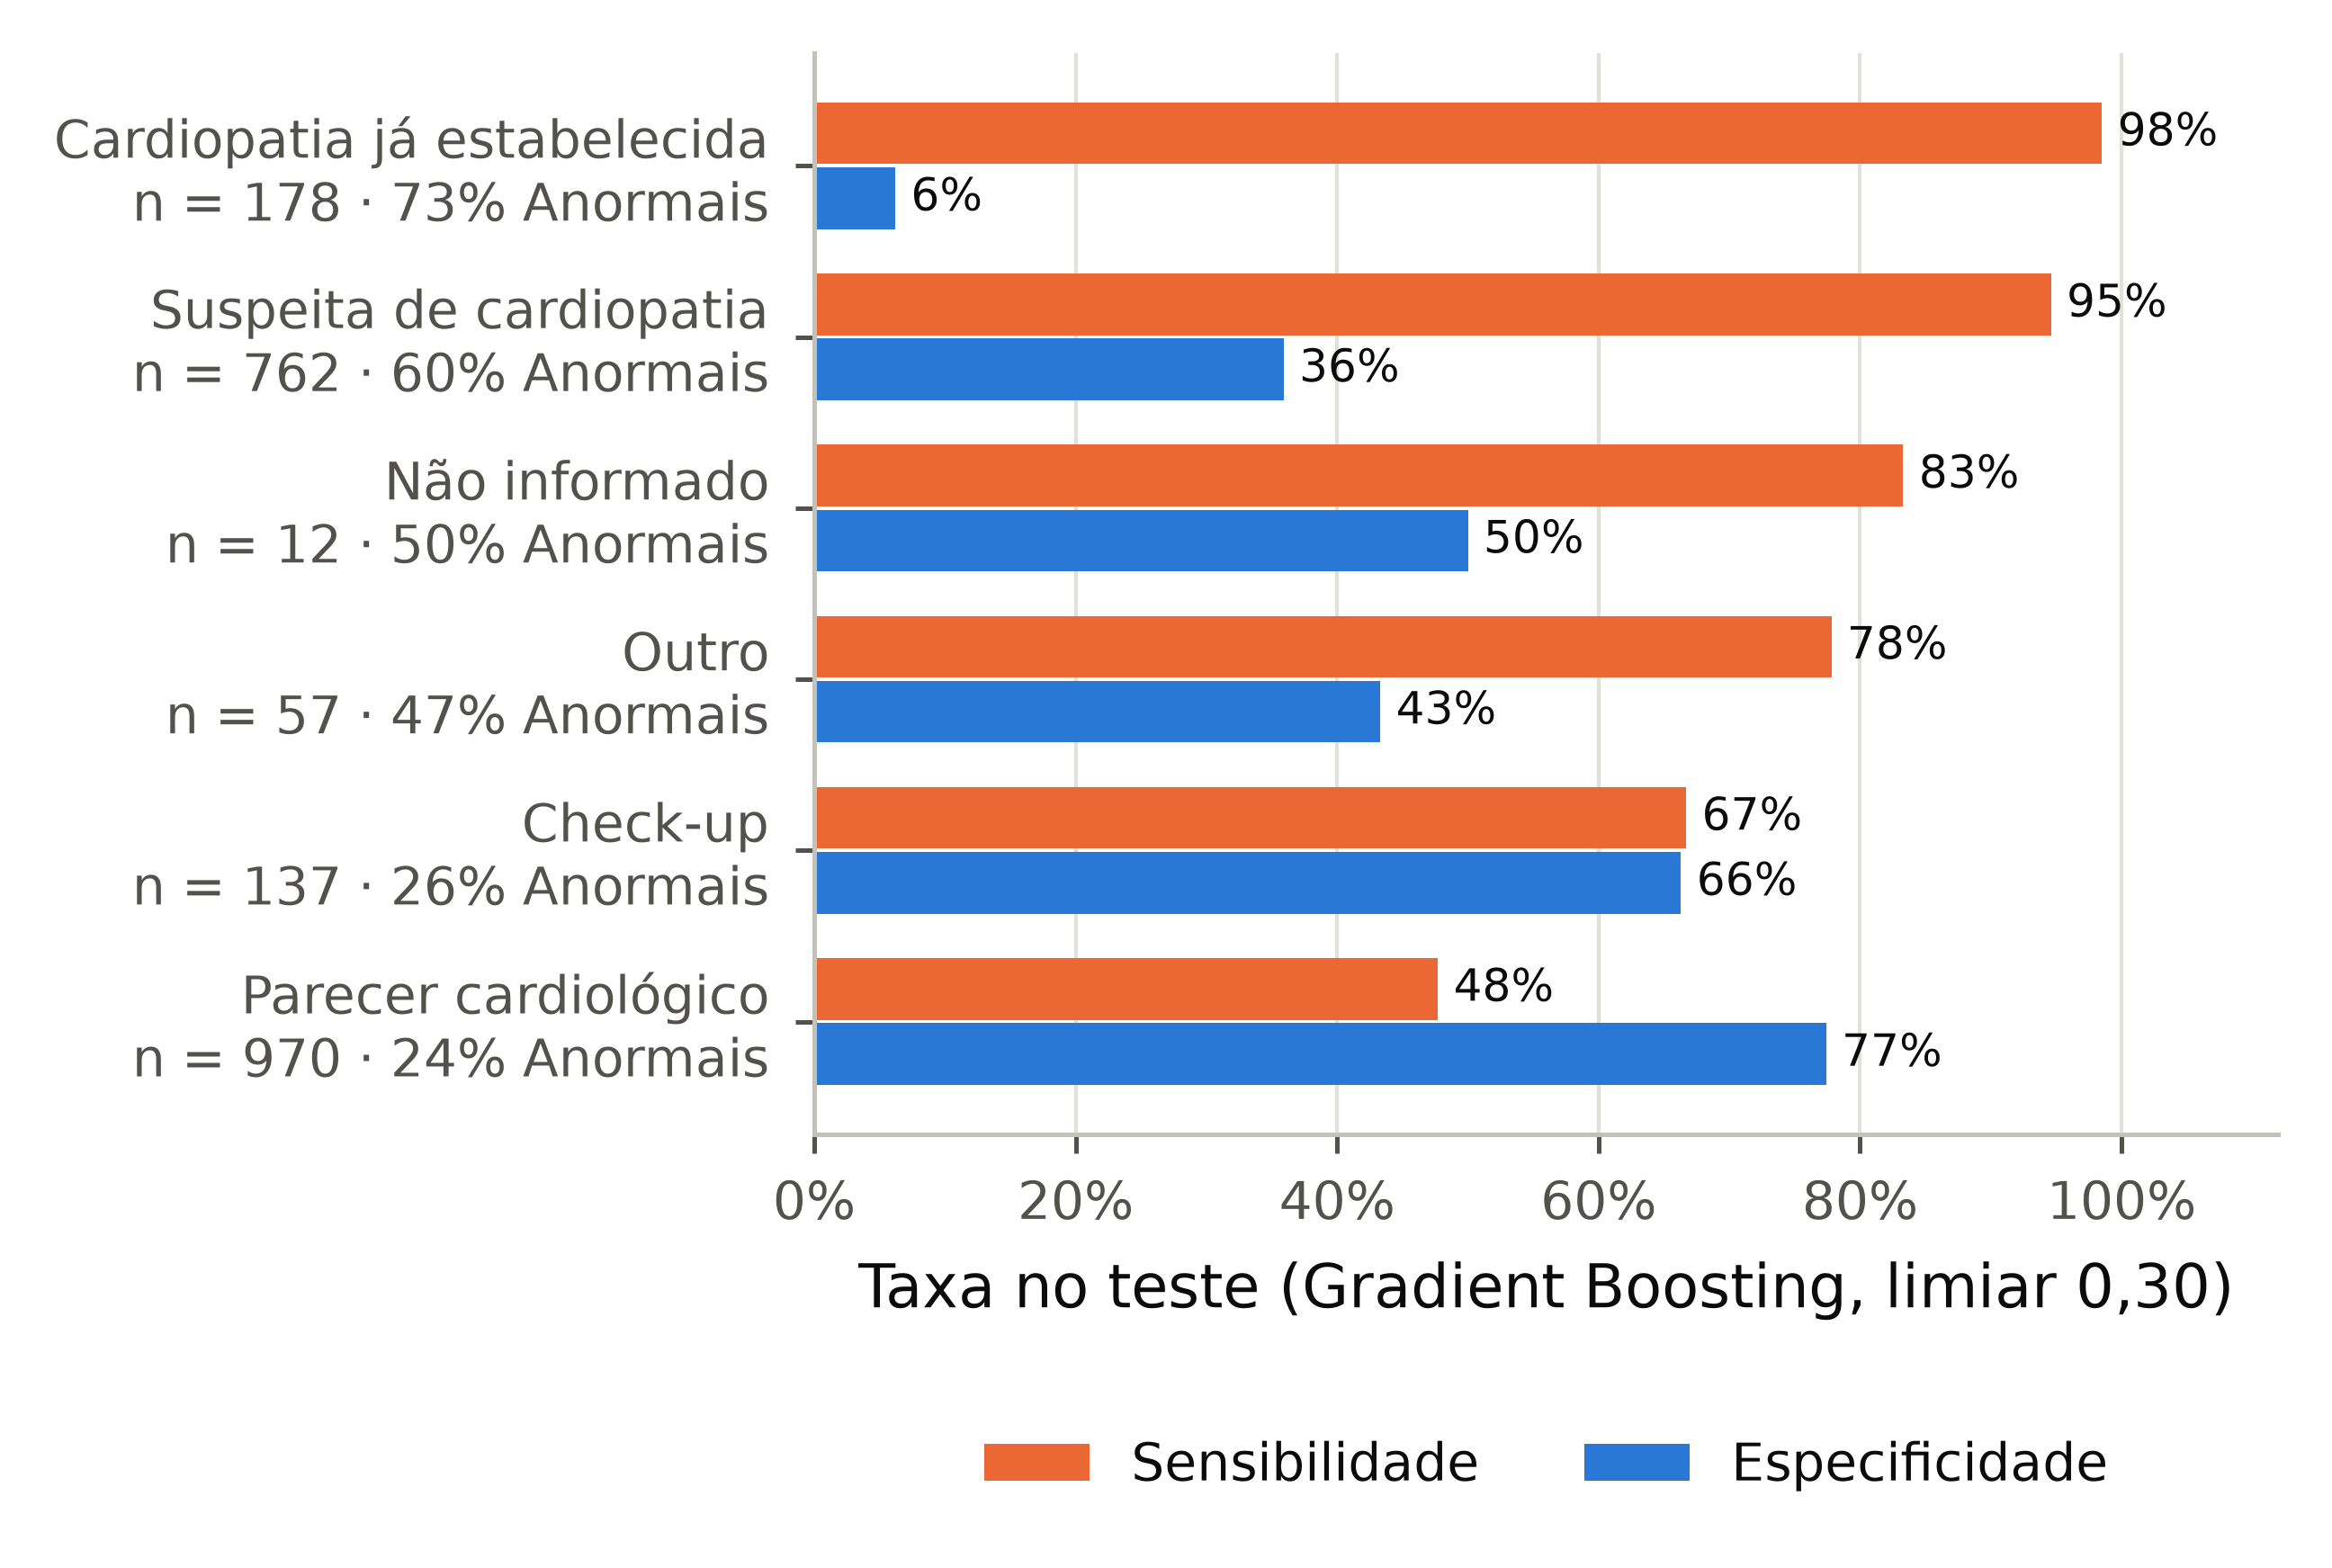
\includegraphics[width=\columnwidth]{fig6_erros_por_motivo}
\caption{Sensibilidade e especificidade do modelo escolhido no conjunto de teste, por motivo principal do encaminhamento, no limiar fixado no treino. Os rótulos trazem o número de consultas e a proporção de laudos anormais de cada grupo.}
\label{fig:fig6_erros_por_motivo}
\end{figure}
\subsection{Importância dos atributos}
A permutação por grupo (Fig. 6) mostra uma concentração acentuada: embaralhar as 18 colunas do motivo do encaminhamento derruba a área sob a curva em 0,204, enquanto nenhum outro grupo passa de 0,028 --- o do grupo ``idade''. Os três modelos concordam na ordenação, o que indica que ela reflete os dados e não a escolha do algoritmo. Individualmente, o atributo mais importante é o encaminhamento por sopro (0,083), seguido pela frequência cardíaca e pela idade.

Os coeficientes da regressão logística dão a direção dos efeitos. Aumentam a chance de laudo anormal os encaminhamentos que já trazem suspeita --- sopro (razão de chances 3,21), cardiopatia já estabelecida (1,94) e cardiopatia congênita (1,76) --- e diminuem os pedidos de rotina, como parecer cardiológico (0,53) e check-up (0,53). A pressão arterial, o índice de massa corporal e o sexo têm efeito desprezível, confirmando o que a análise bivariada da etapa anterior já indicava.

\begin{figure}[!t]
\centering
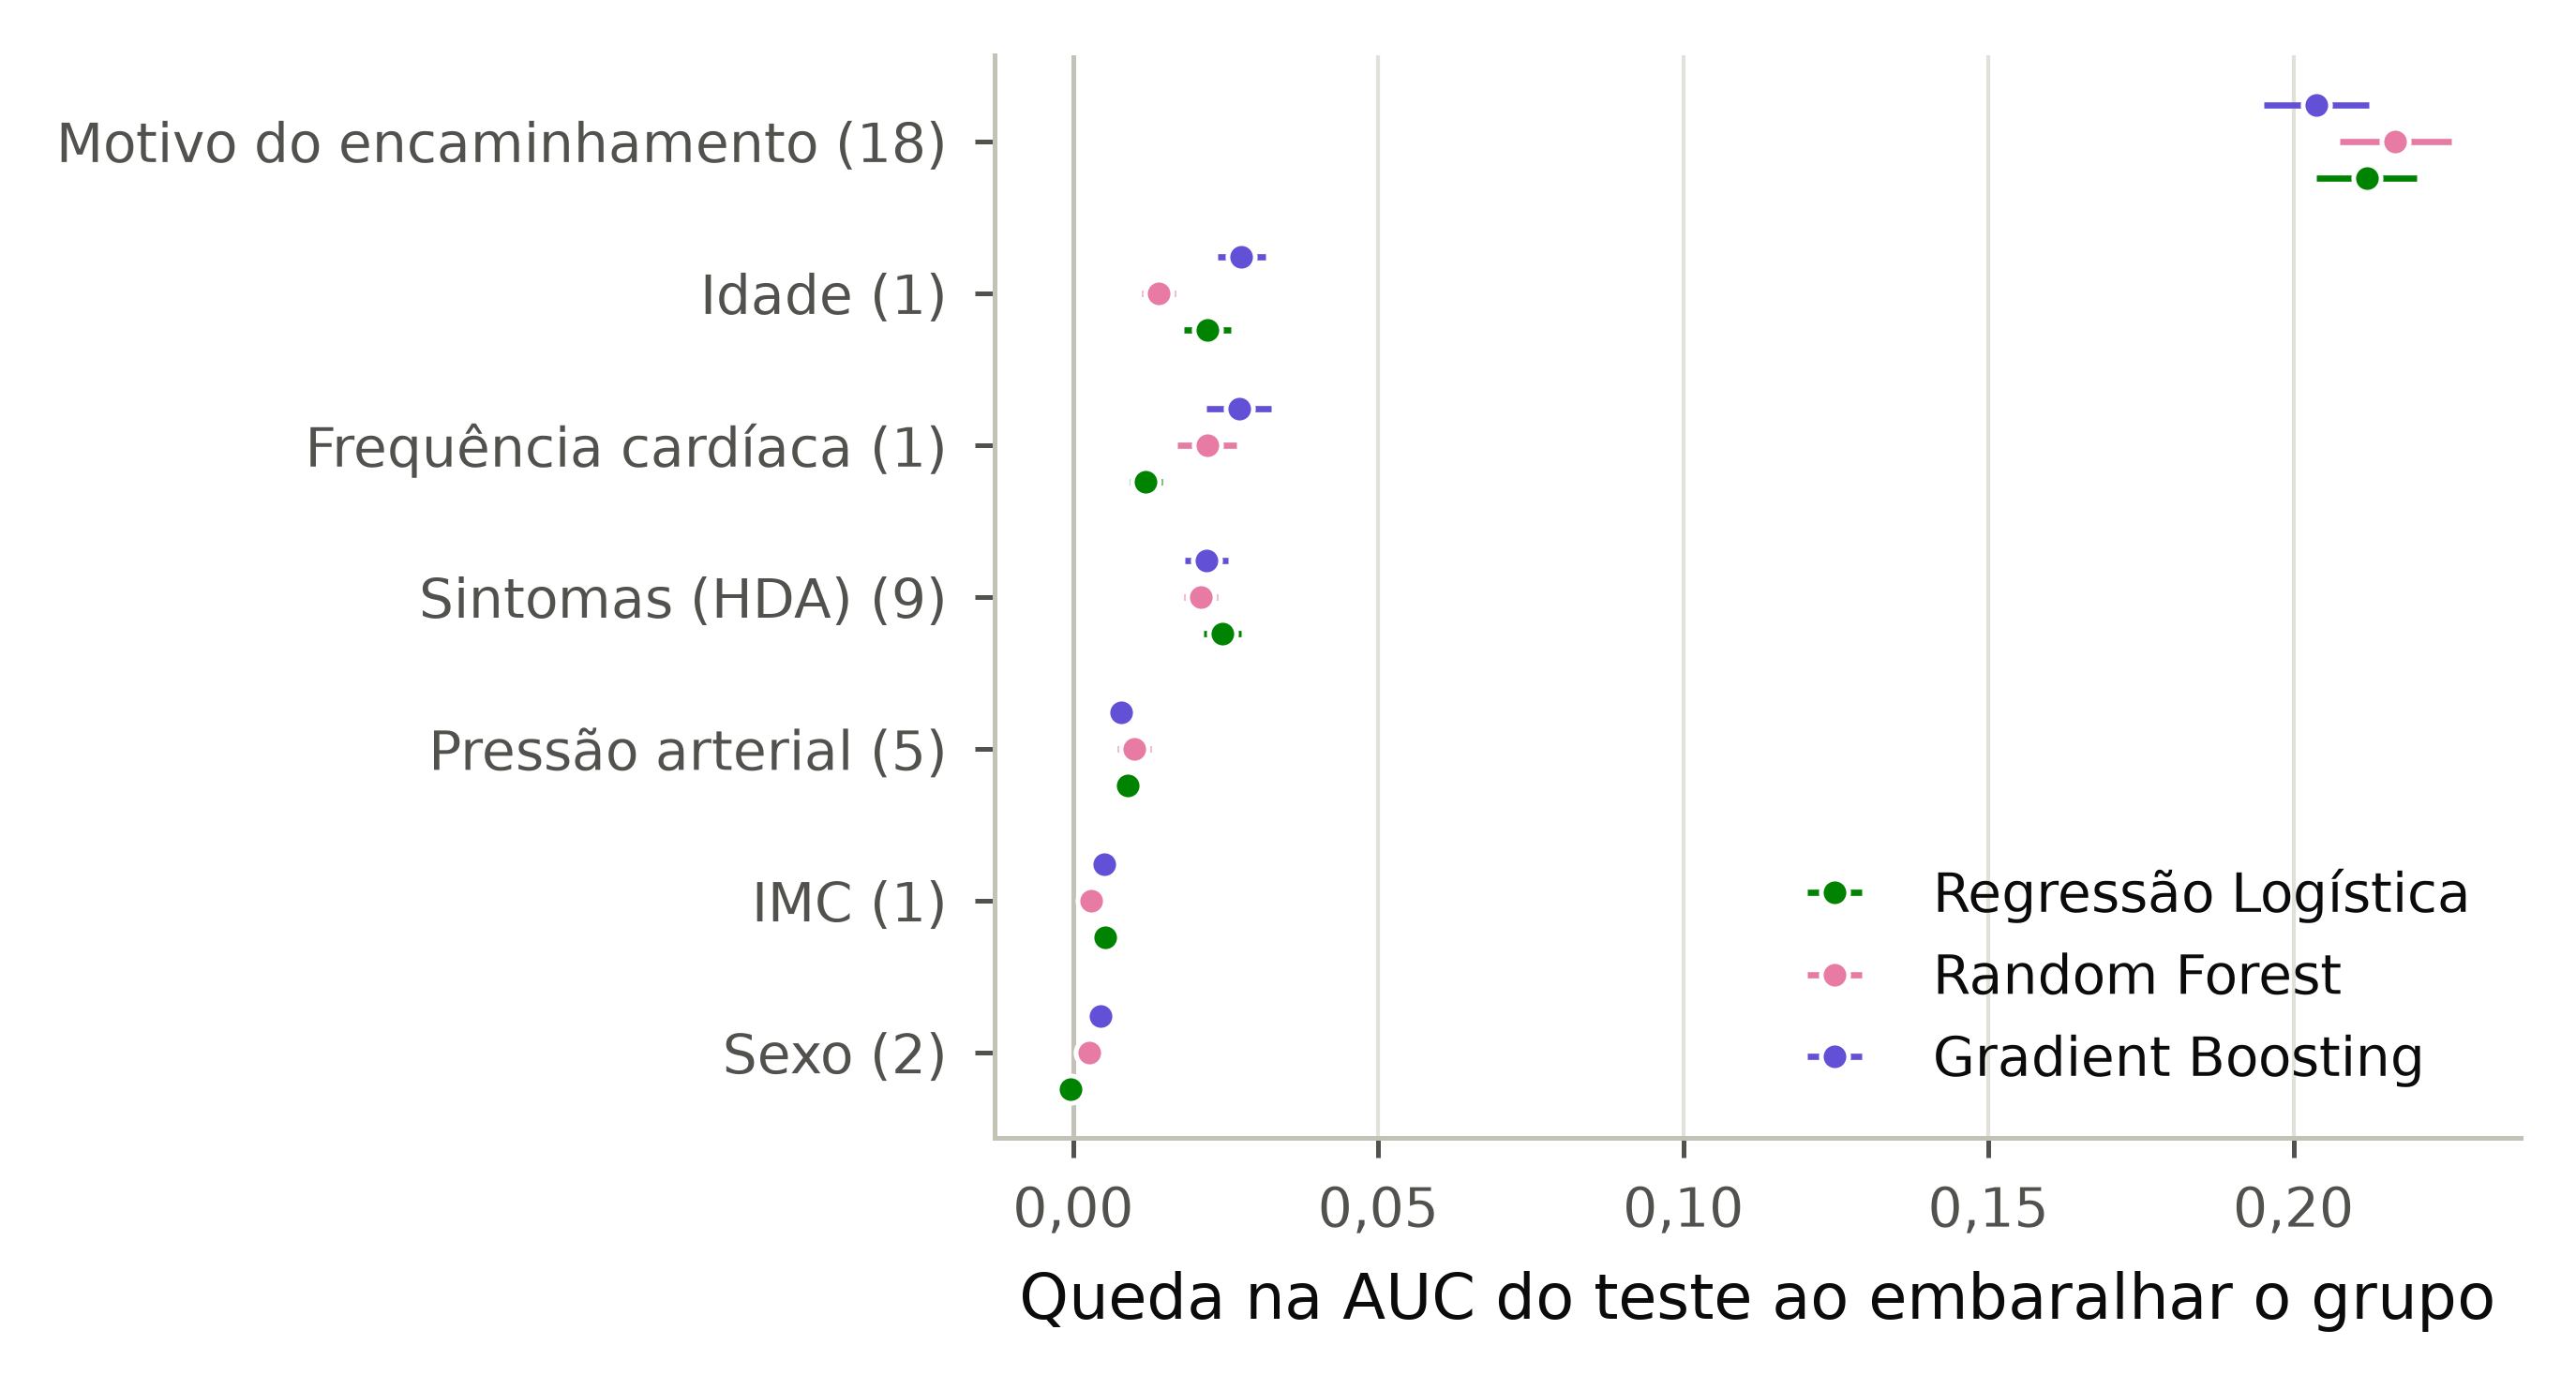
\includegraphics[width=\columnwidth]{fig5_importancia_grupos}
\caption{Queda na área sob a curva ROC do teste ao embaralhar, em conjunto, as colunas de cada grupo temático (média de 30 repetições, barras de desvio-padrão). Entre parênteses, o número de colunas do grupo.}
\label{fig:fig5_importancia_grupos}
\end{figure}
\subsection{Robustez e limitações}
A proporção de laudos anormais diminui ao longo da série histórica, de 55,8\% em 2003 para 28,6\% em 2010, o que sugere mudança no perfil dos atendimentos. Como a validação cruzada sorteia as dobras ao acaso e mistura os anos, o experimento foi repetido com divisão temporal (Tabela IV): treinando nos anos iniciais e validando nos finais, a área sob a curva do gradient boosting fica em 0,764, contra 0,802 no teste sorteado. A capacidade de ordenar resiste; o que muda é a prevalência na validação (37,7\% contra 42,4\% na base), o que desloca o ponto de operação e penaliza a precisão.

\begin{table}[!t]
\caption{Área sob a curva ROC sob dois protocolos: o teste sorteado e uma divisão temporal, que treina nos anos iniciais da série e valida nos finais. A diferença de prevalência entre os dois conjuntos de validação explica parte da variação.}
\label{tab:deriva_temporal}
\centering
\small
\begin{tabular}{llccc}
\toprule
protocolo & valid. (n) & \% An. & logística & boosting \\
\midrule
dobras ao acaso (teste 80/20) & 2.116 & 42,4 & 0,792 & 0,802 \\
treino até 2007, validação de 2008 em diante & 4.497 & 37,7 & 0,771 & 0,764 \\
\bottomrule
\end{tabular}
\end{table}
Três limitações delimitam o alcance destes resultados. A base não possui identificador de paciente, de modo que consultas repetidas da mesma criança, se existirem, não podem ser mantidas do mesmo lado da divisão. O perfil dos atendimentos muda ao longo dos anos, e o desempenho medido vale para a distribuição observada. Por fim, o rótulo é o laudo registrado por um cardiologista, não um desfecho confirmado por exame complementar: o modelo aprende a reproduzir um julgamento clínico, com a variabilidade que lhe é própria.

\section{Conclusão}
A exclusão dos achados do exame físico reduziu a área sob a curva ROC de 0,95 para 0,78, e a validação cruzada aninhada sobre a base completa estima 0,786 para o melhor modelo. Esses dois números, lidos em conjunto, são o resultado do trabalho: o desempenho aparentemente excelente do primeiro cenário vinha de atributos registrados no mesmo ato clínico que gera o rótulo, e o desempenho honesto é moderado.

A diferença entre o melhor modelo complexo e o baseline linear foi de 0,012 de área sob a curva, enquanto a exclusão do exame físico respondeu por 0,174 --- 14 vezes mais. O limite deste problema está na informação disponível antes da consulta, não na escolha do algoritmo --- e em uso clínico a regressão logística seria defensável pela interpretabilidade.

Como triagem, a utilidade é parcial e localizada: o modelo ordena bem as crianças que chegam com suspeita registrada no encaminhamento e é fraco nos pedidos de rotina, onde estão 73\% dos laudos anormais que ele deixa passar. Como continuidade, três caminhos se destacam: incorporar atributos anteriores à consulta que a base não contém, como histórico familiar e dados do pré-natal; tratar o texto livre do encaminhamento, hoje reduzido a categorias; e validar o modelo em outro serviço, para separar o que é padrão clínico do que é característica deste ambulatório.

\section{Uso de Inteligência Artificial Generativa}
O assistente Claude (Anthropic) foi utilizado em quatro frentes, sempre a partir do protocolo definido pelo grupo: organização do repositório e da documentação; escrita do código de modelagem e das figuras; verificação da suposição de agrupamento por paciente descrita na Seção III-B, que resultou na correção aqui adotada; e redação deste relatório a partir das tabelas geradas pela execução do código. Nenhum número apresentado foi produzido pelo assistente: todos são lidos dos arquivos exportados pela execução, e o relatório é gerado por um programa que os consulta. As decisões metodológicas --- quais atributos excluir, qual protocolo de validação adotar, quais algoritmos comparar e qual ponto de operação considerar --- foram tomadas pelo grupo e estão registradas no repositório.

\begin{thebibliography}{00}
\bibitem{b1} F. Pedregosa et al., ``Scikit-learn: Machine learning in Python'', Journal of Machine Learning Research, vol. 12, pp. 2825--2830, 2011.
\bibitem{b2} The pandas development team, ``pandas-dev/pandas: Pandas'', Zenodo, 2024. [Online]. Disponível em: https://doi.org/10.5281/zenodo.3509134
\bibitem{b3} J. D. Hunter, ``Matplotlib: A 2D graphics environment'', Computing in Science \& Engineering, vol. 9, no. 3, pp. 90--95, 2007.
\bibitem{b4} R. J. Kuczmarski et al., ``2000 CDC growth charts for the United States: methods and development'', Vital and Health Statistics, series 11, no. 246, National Center for Health Statistics, 2002.
\bibitem{b5} National High Blood Pressure Education Program Working Group on High Blood Pressure in Children and Adolescents, ``The fourth report on the diagnosis, evaluation, and treatment of high blood pressure in children and adolescents'', Pediatrics, vol. 114, no. 2, pp. 555--576, 2004.
\bibitem{b6} American Academy of Pediatrics, Council on Child and Adolescent Health, ``Age limits of pediatrics'', Pediatrics, vol. 81, no. 5, p. 736, 1988.
\bibitem{b7} S. Varma e R. Simon, ``Bias in error estimation when using cross-validation for model selection'', BMC Bioinformatics, vol. 7, no. 91, 2006.
\bibitem{b8} S. Kaufman, S. Rosset e C. Perlich, ``Leakage in data mining: formulation, detection, and avoidance'', ACM Transactions on Knowledge Discovery from Data, vol. 6, no. 4, pp. 1--21, 2012.
\bibitem{b9} L. Breiman, ``Random forests'', Machine Learning, vol. 45, no. 1, pp. 5--32, 2001.
\bibitem{b10} J. H. Friedman, ``Greedy function approximation: a gradient boosting machine'', The Annals of Statistics, vol. 29, no. 5, pp. 1189--1232, 2001.
\bibitem{b11} B. Efron e R. J. Tibshirani, An Introduction to the Bootstrap. New York: Chapman \& Hall, 1993.
\end{thebibliography}
\end{document}